\documentclass{article}
\usepackage[a4paper, margin=1in]{geometry}
\usepackage{graphicx} % Required for inserting 
\usepackage{subcaption}
\usepackage{geometry}
\usepackage{amsmath}
\usepackage{amsfonts}
\usepackage{amssymb}
\usepackage{hyperref}
\usepackage{float}

\documentclass{article}
\usepackage{graphicx} % Required for inserting images
\usepackage{amsmath}
\usepackage{amssymb}
\usepackage{graphicx}
\usepackage{geometry}
\geometry{margin=1in}
\usepackage[table,xcdraw]{xcolor}




\begin{document}



\begin{titlepage}
    \centering
    \vspace*{1cm}
    
    \Huge
    \textbf{CSE 306} \\[0.5cm]
    \LARGE
    Computer Architecture Sessional \\[1.5cm]
    
    \Large
    \textbf{Assignment-2: 32-bit Floating Point Adder Simulation} \\[2cm]
    
    \large
    Section - B2 \\[0.3cm]
    Group - 02 \\[2cm]
    
    \Large
    \textbf{Members of the Group:} \\[1cm]
    
    \normalsize
    \begin{itemize}
        \item[i] 2105091 - Shemanty Mahjabin
        \item[ii] 2105096 - Fabliha Afia
        \item[iii] 2105103 - Mahabuba Sharmin Mim
     \end{itemize}    
    
    \vfill
    
\end{titlepage}
\section{Introduction}

Floating-point arithmetic is a critical component in computer architecture, enabling the representation and manipulation of real numbers with varying degrees of precision. In this assignment, the objective is to design a floating-point adder circuit that takes two 32-bit floating-point numbers as input and outputs their sum, adhering to the IEEE 754 standard. This standard divides a floating-point number into three components: the sign bit, the exponent, and the fraction (or mantissa), allowing efficient representation and calculations across a wide range of values.

The addition process involves several key steps. First, the circuit must align the inputs by adjusting the exponents through shifting, ensuring the mantissas can be added directly. Post addition, normalization is performed to restore the result to its proper form, and rounding ensures precision within the constraints of the 32-bit representation. Special conditions, such as overflow, underflow, and zero handling, are accounted for, enhancing the circuit's reliability.

This floating-point adder finds practical applications in diverse fields, including scientific computing, graphics rendering, and machine learning, where high-speed and high-precision arithmetic operations are essential. While modern simulators provide tools like prebuilt arithmetic logic units (ALUs) and shifters, constructing the logic at a modular level ensures an in-depth understanding of the design principles.

The outcome of this assignment will include a detailed implementation of the floating-point addition process, emphasizing modularity, correctness, and adherence to IEEE standards. This report will document the design methodology, algorithm flow, architectural design, and simulation results, providing a comprehensive overview of the system.


\section{Problem Specification}

The task involves creating a circuit for a floating-point adder that accepts two floating-point numbers as inputs, computes their sum, and outputs another floating-point number. Each floating-point number will have a length of 32 bits and will be represented as follows:

\begin{center}
    \begin{tabular}{|c|c|c|}
        \hline
        \textbf{Sign} & \textbf{Exponent} & \textbf{Fraction} \\ \hline
        1 bit         & 9 bits           & 22 bits           \\ \hline
    \end{tabular}
\end{center}


\section{ Description and Circuit Diagram of Modules}

To ensure modularity in the design of the floating-point adder, several specialized libraries have been developed and implemented. Below are the descriptions and uses of these libraries.

\subsection*{Input Splitter}
This module splits a 32-bit floating-point number into three parts:
\begin{itemize}
    \item \textbf{1-bit sign}: Determines the sign of the number (positive or negative).
    \item \textbf{11-bit exponent}: Encodes the exponent value for the floating-point representation.
    \item \textbf{20-bit fraction}: Represents the significand (or mantissa) of the number.
\end{itemize}
The Input Splitter ensures proper segmentation of the input for subsequent processing steps.

\begin{figure}[h!]
\centering
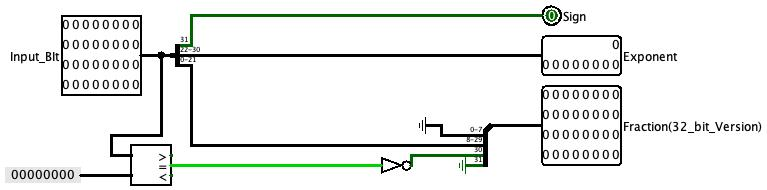
\includegraphics[width=0.8\textwidth]{Input_splitter.jpg} % Replace with actual image filename
\caption{Input Splitter module.}
\label{fig:input_splitter}
\end{figure}


\subsection{Adder Library}

An adder circuit (\texttt{adder32bit.circ}) has been included in the \texttt{adder32bit} library, which performs the most crucial part of the Floating Point Adder (FPA) by adding the significands of the two given input floating-point numbers.

\begin{figure}[H]
    \centering
    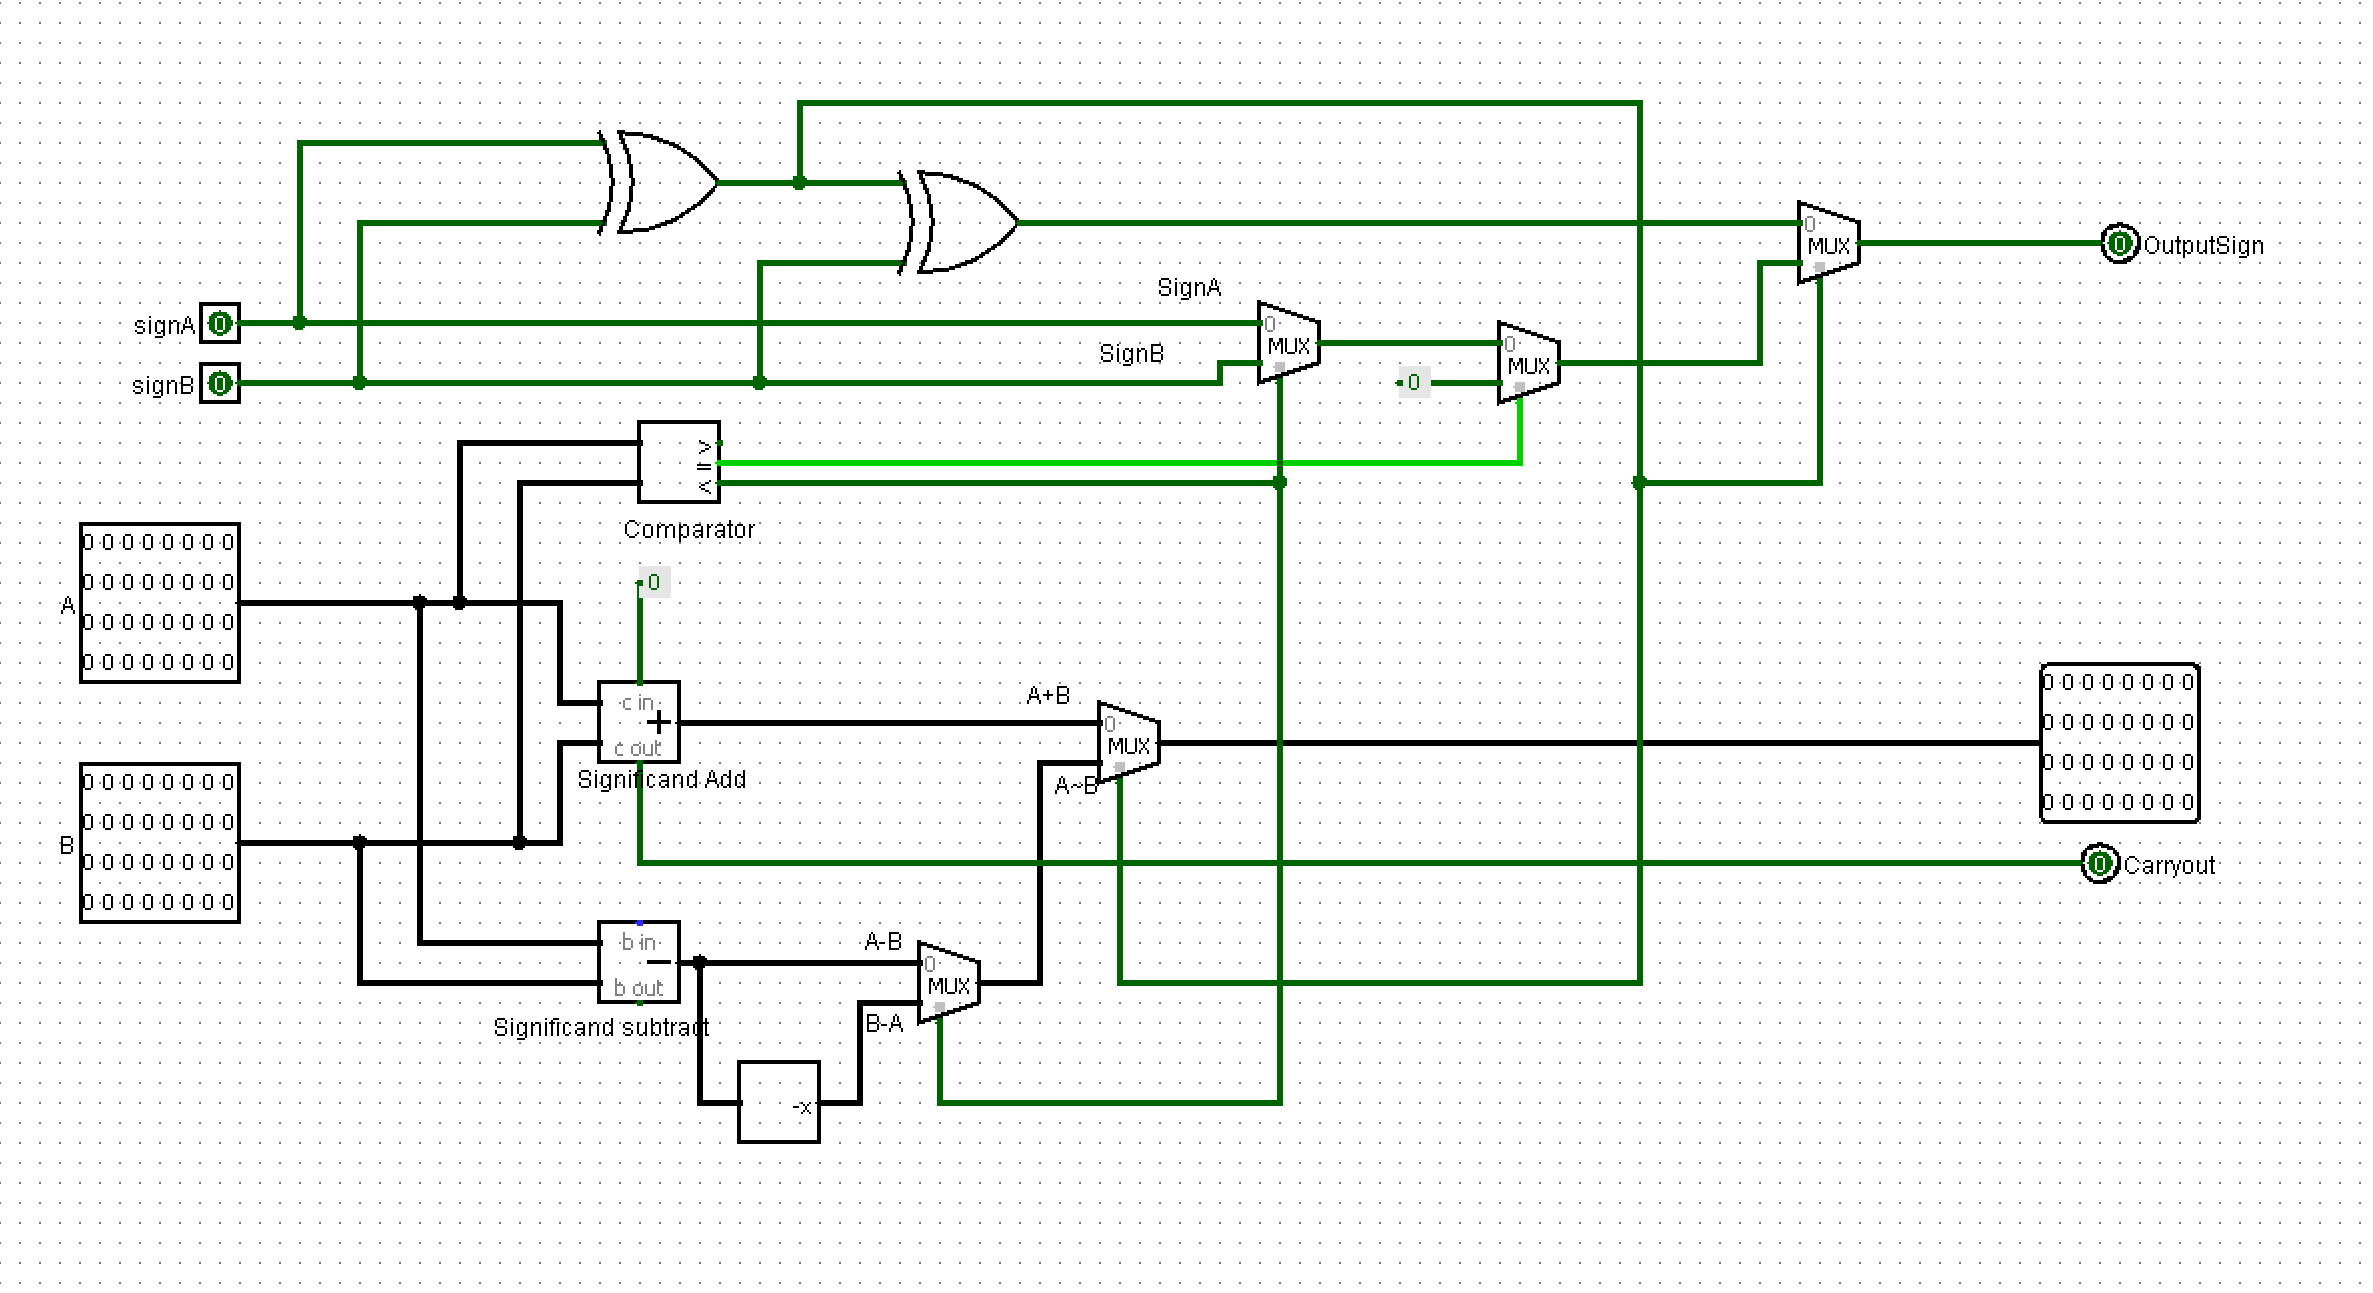
\includegraphics[width=0.8\textwidth]{32bit_adder_circuit.png} % Replace with your image file name
    \caption{32 Bit Adder Circuit}
    \label{fig:32bit_adder}
\end{figure}


\subsection{ Shifter Library}

Shifters are required in floating-point adders to shift the fraction in order to normalize or balance with the other operand. We have implemented shifters (\texttt{leftShifterLib.circ} and \texttt{rightShifterLib.circ}) with splitters and multiplexers (muxes) from the Logisim built-in library. The circuits in the libraries are:

\begin{itemize}
    \item \textbf{1, 2, 4, 8, 16 bits left shifter:} \texttt{1LeftShift}, \texttt{2LeftShift}, \texttt{4LeftShift}, \texttt{8LeftShift}, \texttt{16LeftShift}
    \item \textbf{1, 2, 4, 8, 16 bits right shifter:} \texttt{1RightShift}, \texttt{2RightShift}, \texttt{4RightShift}, \texttt{8RightShift}, \texttt{16RightShift}
    \item \textbf{Arbitrary left and right shifter:} (Can shift any number of bits up to 31 bits) \texttt{ArbLeftShift}, \texttt{ArbRightShift}
    \item \textbf{Right shifter that will make every bit 0 if it needs shifting more than 31 bits:} \texttt{RightShiftWithEmpty}
\end{itemize}


\begin{figure}[H]
    \centering
    % Row 1
    \begin{subfigure}[b]{0.3\textwidth}
        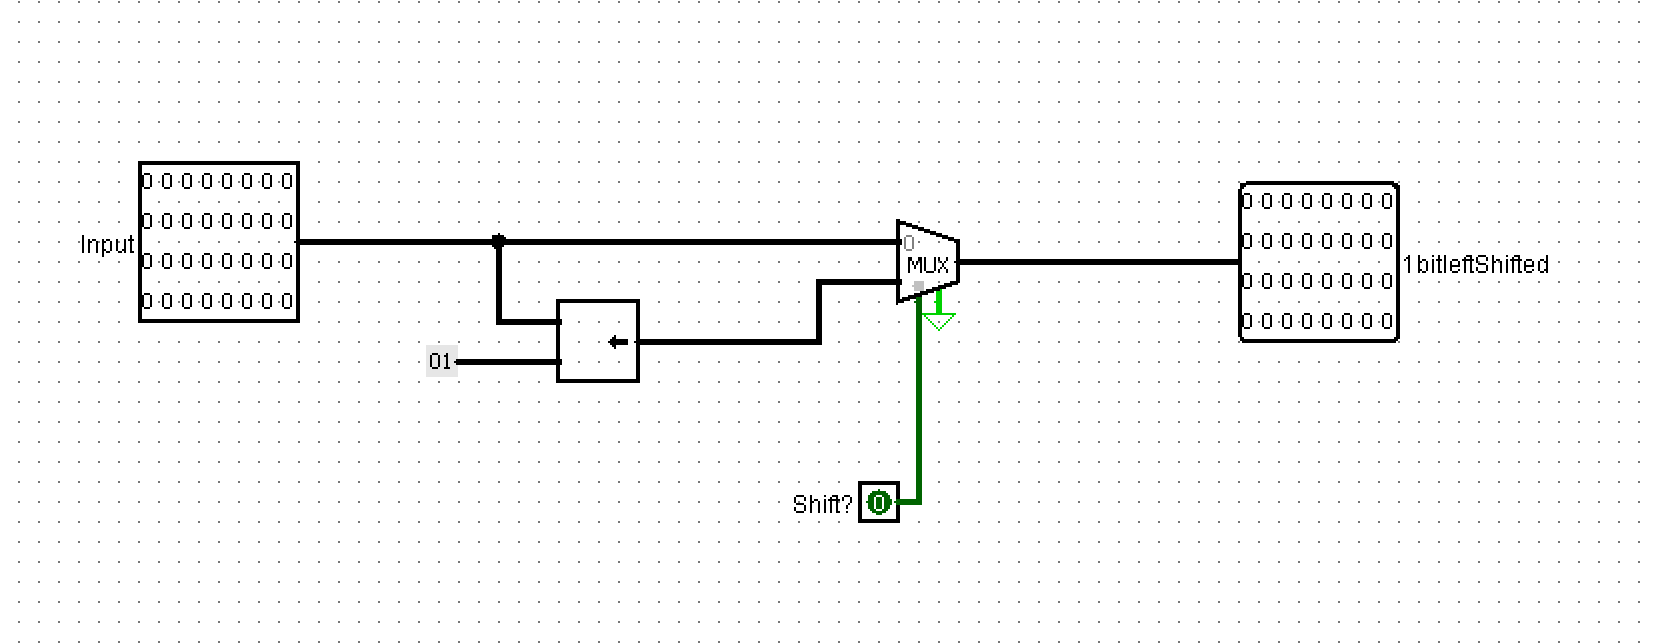
\includegraphics[width=\textwidth]{1bitleftshifter.png} % Replace with your image file
        \caption{1 Bit Left Shifter}
        \label{fig:1bit}
    \end{subfigure}
    \hfill
    \begin{subfigure}[b]{0.3\textwidth}
        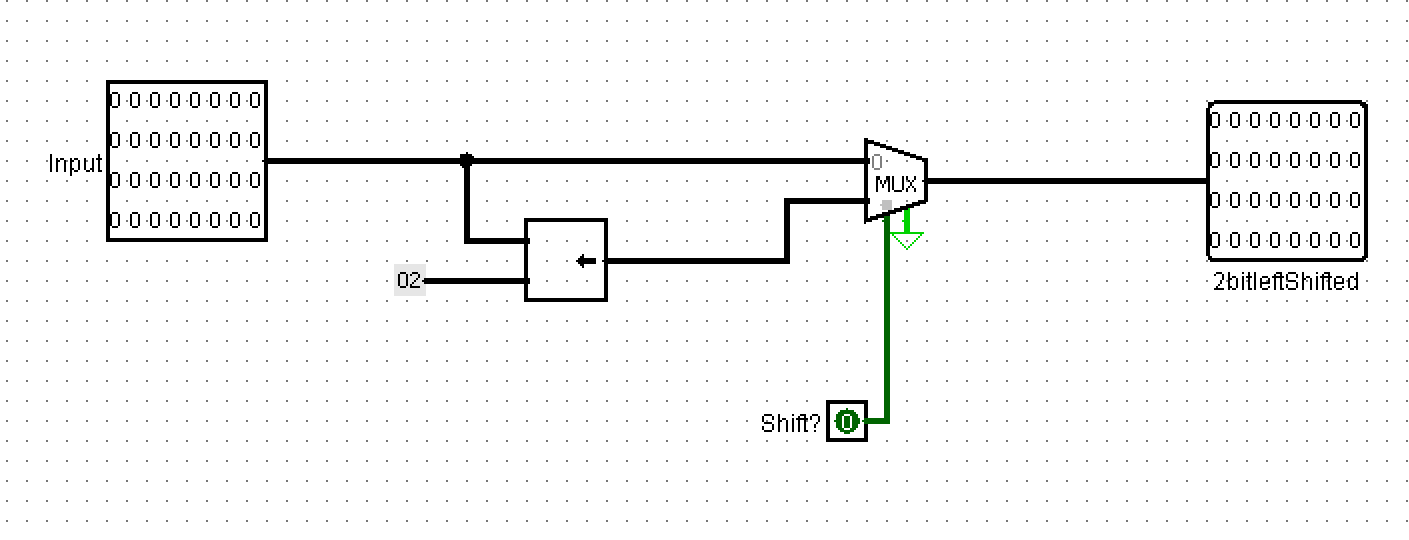
\includegraphics[width=\textwidth]{2bitleftshifter.png} % Replace with your image file
        \caption{2 Bit Left Shifter}
        \label{fig:2bit}
    \end{subfigure}
    \hfill
    \begin{subfigure}[b]{0.3\textwidth}
        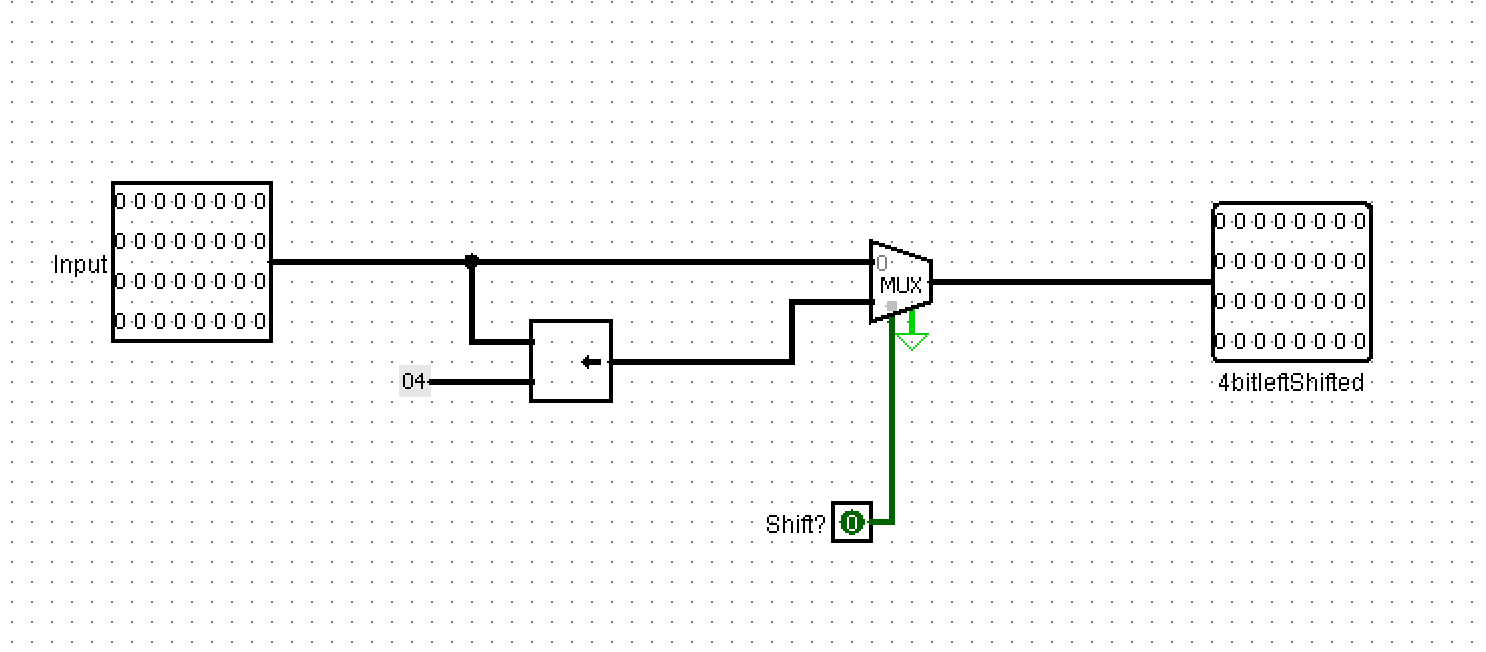
\includegraphics[width=\textwidth]{4bitleftshifter.png} % Replace with your image file
        \caption{4 Bit Left Shifter}
        \label{fig:4bit}
    \end{subfigure}

    \vspace{1em} % Adjust spacing between rows

    % Row 2
    \begin{subfigure}[b]{0.3\textwidth}
        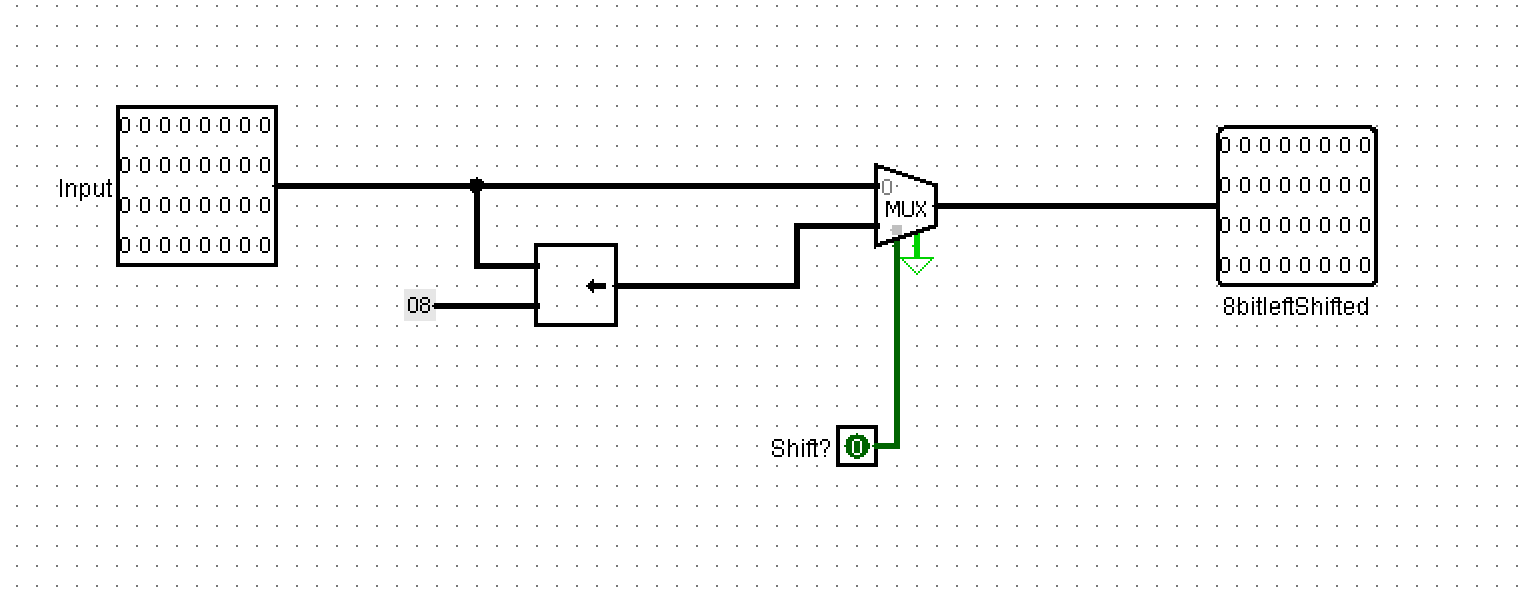
\includegraphics[width=\textwidth]{8bitleftshifter.png} % Replace with your image file
        \caption{8 Bit Left Shifter}
        \label{fig:8bit}
    \end{subfigure}
    \hfill
    \begin{subfigure}[b]{0.3\textwidth}
        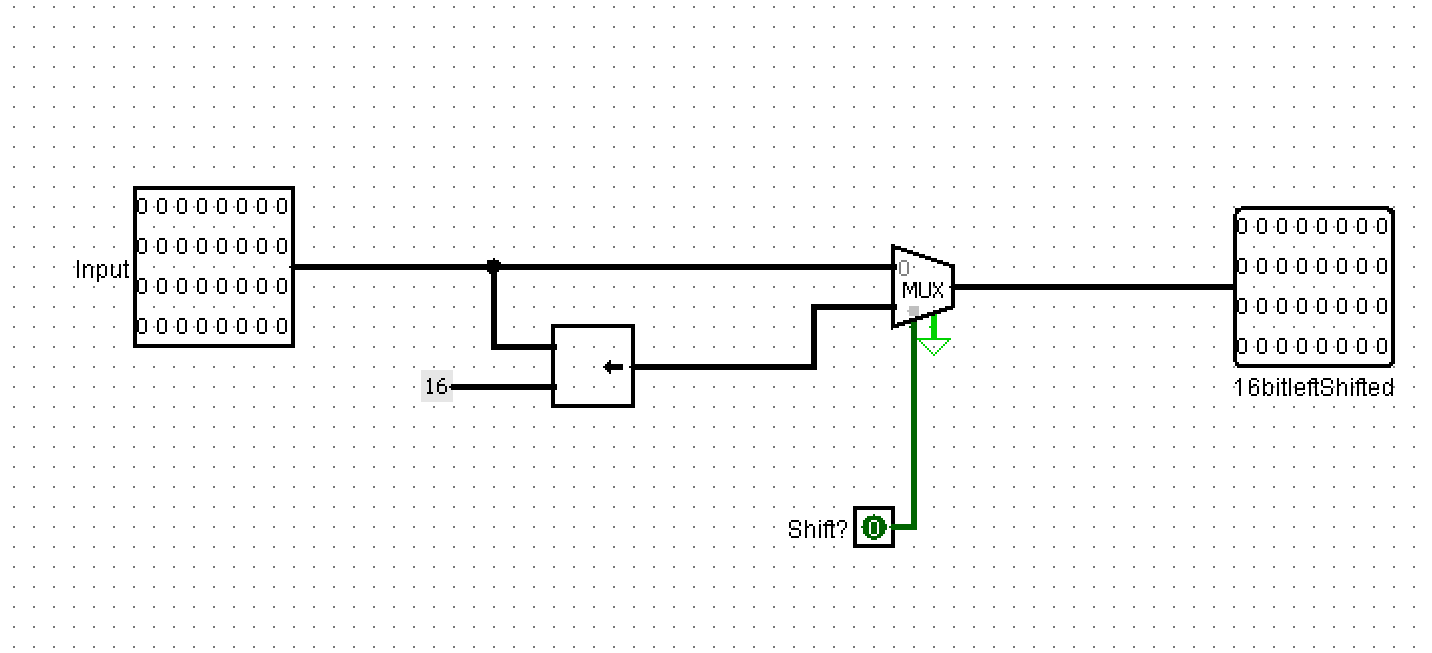
\includegraphics[width=\textwidth]{16bitleftshifter.png} % Replace with your image file
        \caption{16 Bit Left Shifter}
        \label{fig:16bit}
    \end{subfigure}
    \hfill
    \begin{subfigure}[b]{0.3\textwidth}
        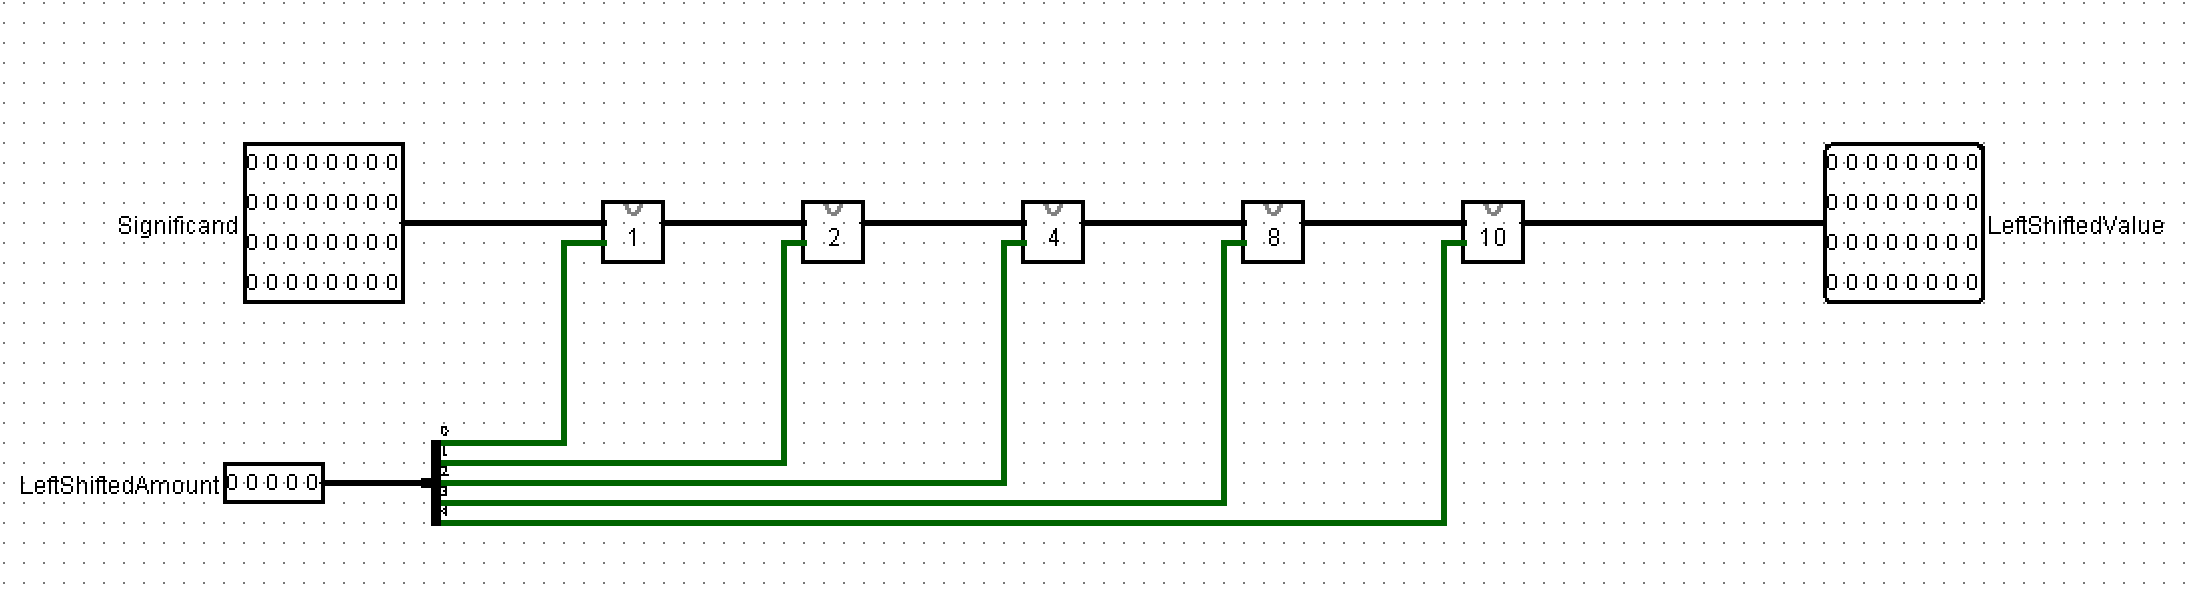
\includegraphics[width=\textwidth]{arbitaryleftshifter.png} % Replace with your image file
        \caption{Arbitrary Left Shifter}
        \label{fig:arb}
    \end{subfigure}
    
    \caption{Shifter Circuits}
    \label{fig:Shifter Circuits}
\end{figure}


\begin{itemize}
    \item \textbf{Left Shifters:} 
    \begin{itemize}
        \item 1-bit left shifter (\texttt{1LeftShift})
        \item 2-bit left shifter (\texttt{2LeftShift})
        \item 4-bit left shifter (\texttt{4LeftShift})
        \item 8-bit left shifter (\texttt{8LeftShift})
        \item 16-bit left shifter (\texttt{16LeftShift})
    \end{itemize}
    
    \item \textbf{Right Shifters:} 
    \begin{itemize}
    \item 1-bit right shifter (\texttt{1\_bit\_right\_shift})
    \item 2-bit right shifter (\texttt{2\_bit\_right\_shift})
    \item 4-bit right shifter (\texttt{4\_bit\_right\_shift})
    \item 8-bit right shifter (\texttt{8\_bit\_right\_shift})
    \item 16-bit right shifter (\texttt{16\_bit\_right\_shift})
\end{itemize}


    \item \textbf{Arbitrary Shifters:} 
    These shifters can handle any bit shift operation from 1 to 31 bits.
    \begin{itemize}
        \item Arbitrary left shifter (\texttt{ArbLeftShift})
        \item Arbitrary right shifter (\texttt{Arbitary\_right\_shifter})
    \end{itemize}
    
    \item \textbf{Special Right Shifter:} 
    This right shifter ensures that any shifting greater than 31 bits results in all bits being set to 0.
    \begin{itemize}
        \item Right shifter with overflow handling (\texttt{right\_shift})
    \end{itemize}
\end{itemize}
\begin{figure}[h!]
\centering
\begin{minipage}{0.3\textwidth}
    \centering
    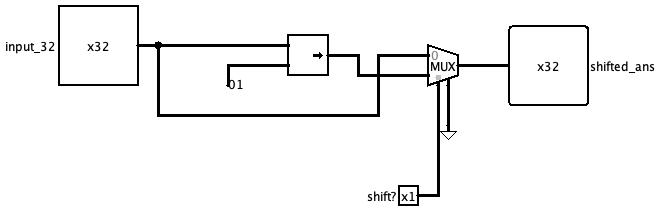
\includegraphics[width=\linewidth]{1bit.jpg}
    1 Bit Right Shifter
    \label{fig:1_bit_right_shift}
\end{minipage} 
\hfill
\begin{minipage}{0.3\textwidth}
    \centering
    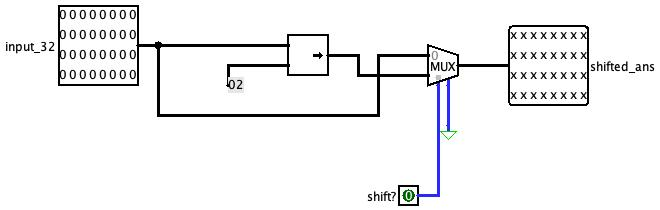
\includegraphics[width=\linewidth]{2.jpg}
    2 Bit Right Shifter
    \label{fig:2_bit_right_shift}
\end{minipage} 
\hfill
\begin{minipage}{0.3\textwidth}
    \centering
    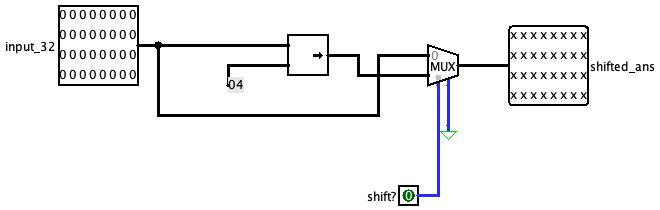
\includegraphics[width=\linewidth]{4.jpg}
    4 Bit Right Shifter
    \label{fig:4_bit_right_shift}
\end{minipage} 
\\
\vspace{0.5cm}
\begin{minipage}{0.3\textwidth}
    \centering
    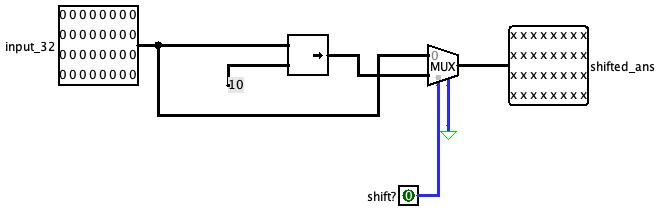
\includegraphics[width=\linewidth]{8.jpg}
    8 Bit Right Shifter
    \label{fig:8_bit_right_shift}
\end{minipage} 
\hfill
\begin{minipage}{0.3\textwidth}
    \centering
    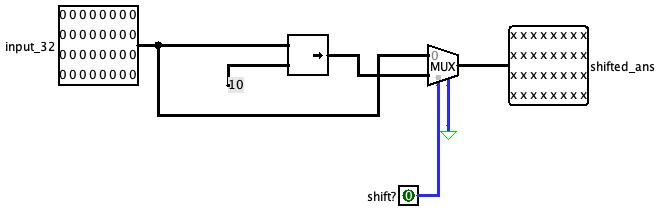
\includegraphics[width=\linewidth]{16.jpg}
    16 Bit Right Shifter
    \label{fig:16_bit_right_shift}
\end{minipage} 
\hfill
\begin{minipage}{0.3\textwidth}
    \centering
    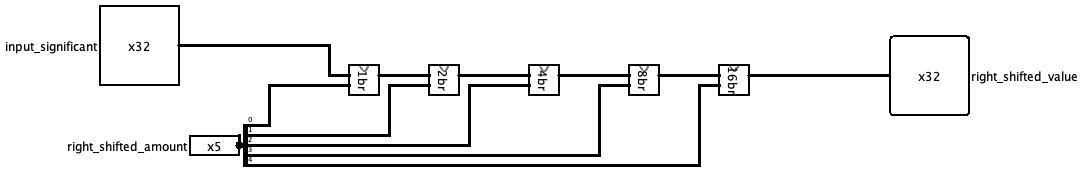
\includegraphics[width=\linewidth]{a.png}
    Arbitrary Right Shifter
    \label{fig:arbitrary_right_shift}
\end{minipage} 
\caption{Shifters used in the design}
\label{fig:shifters}
\end{figure}

% For the second image, the one with the right shift with empty
\begin{figure}[h!]
\centering
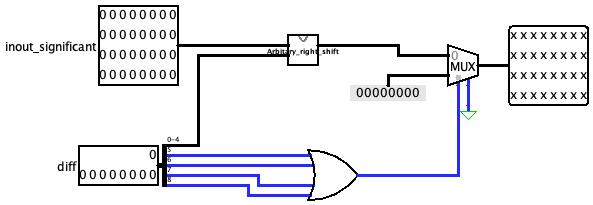
\includegraphics[width=0.6\textwidth]{r.jpg}  % Make the final image smaller
\caption{Right Shift With Empty}
\label{fig:right_shift_with_empty}
\end{figure}



\subsection*{3.4 Normalization Library}

The normalization process in the floating-point adder is handled using a specialized library designed to align and adjust the mantissa and exponent for accurate computation. This library includes a set of components that collaboratively manage the normalization steps by determining the necessary bit shifts and performing adjustments to ensure the final output adheres to the IEEE 754 format. Additionally, an 11-bit value is produced and added to the exponent during this process to ensure proper scaling.

The components of the normalization library are as follows:
\begin{itemize}
    \item \textbf{Normalizer:} Aligns the inputs and ensures proper scaling by managing shifts and adjustments.
    \item \textbf{Shifter:} Performs precise bit-level shifting operations to align the mantissas before addition.
    \item \textbf{Adder-Subtractor:} Facilitates the addition or subtraction of values during exponent adjustments.
    \item \textbf{Rounded Normalizer:} Handles rounding of results to ensure precision within the 32-bit constraints.
    \item \textbf{Zero-Checker:} Detects if the result is zero and appropriately handles such scenarios.
    \item \textbf{One-Checker:} Verifies specific conditions related to exponent values to maintain accuracy.
\end{itemize}

This library simplifies the implementation process by breaking down the normalization into modular subcomponents, making the overall design more efficient and easier to debug.

\begin{figure}[h!]
    \centering
    \begin{subfigure}[b]{0.3\textwidth}
        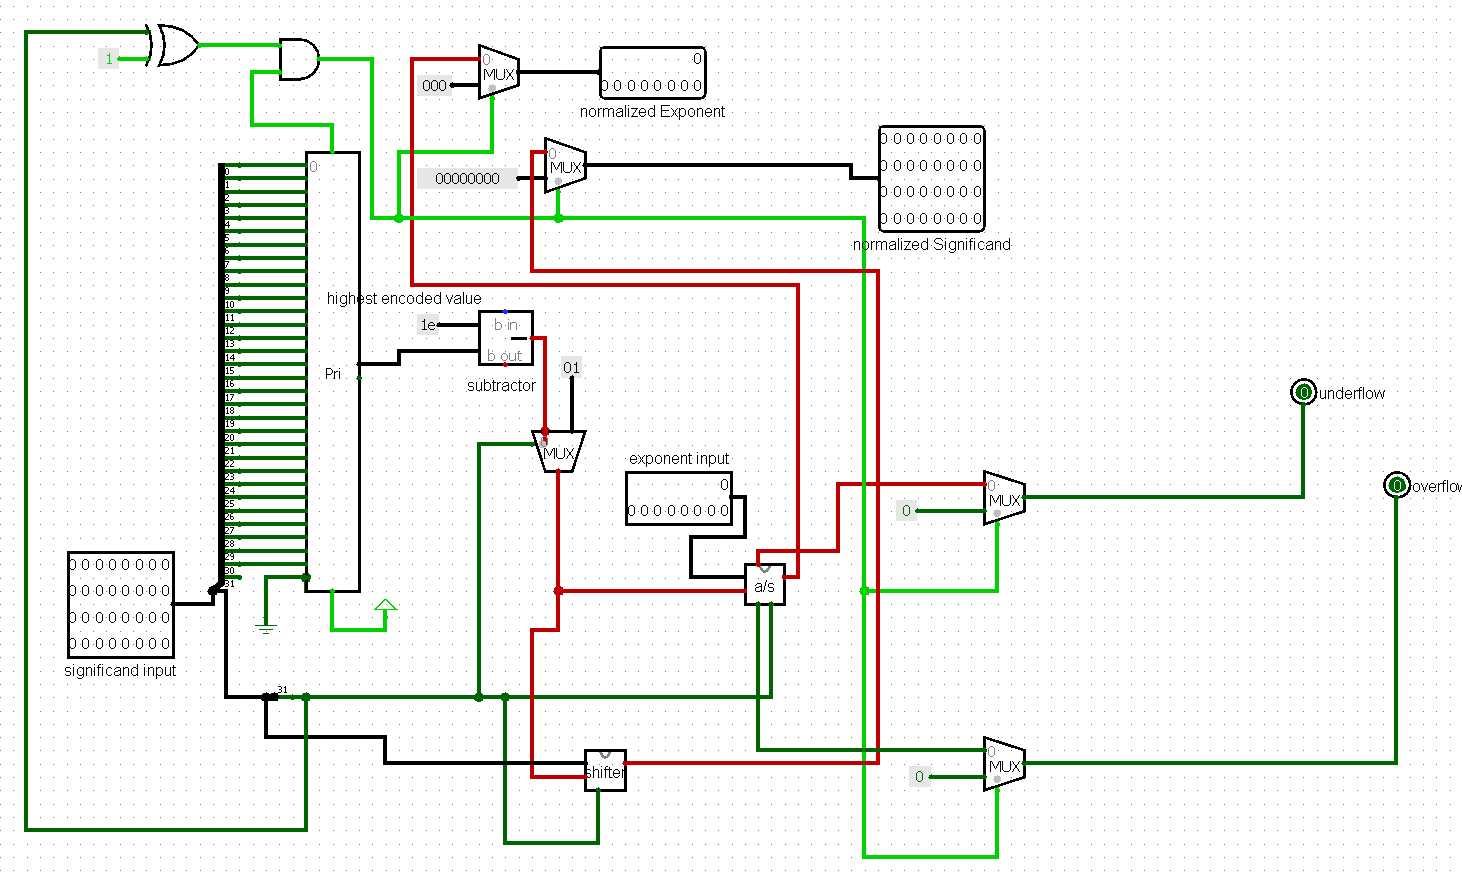
\includegraphics[width=\textwidth]{Normalizer.png}
        \caption{Normalizer}
    \end{subfigure}
    \begin{subfigure}[b]{0.3\textwidth}
        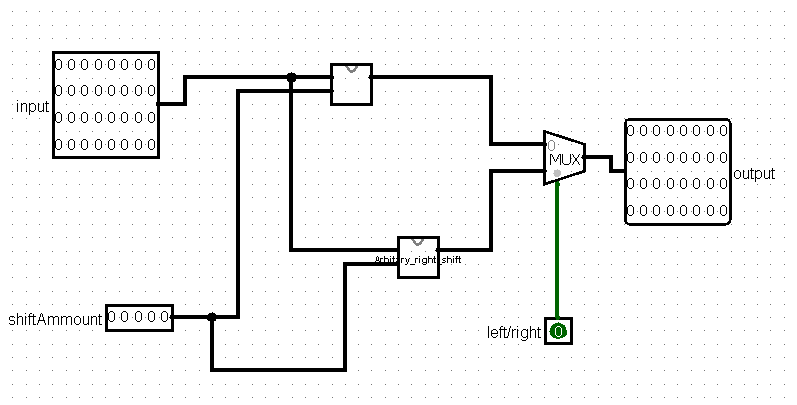
\includegraphics[width=\textwidth]{Shifter.png}
        \caption{Shifter}
    \end{subfigure}
    \begin{subfigure}[b]{0.3\textwidth}
        \includegraphics[width=\textwidth]{adder_subtractor.png}
        \caption{Adder-Subtractor}
    \end{subfigure}
    
    \begin{subfigure}[b]{0.3\textwidth}
        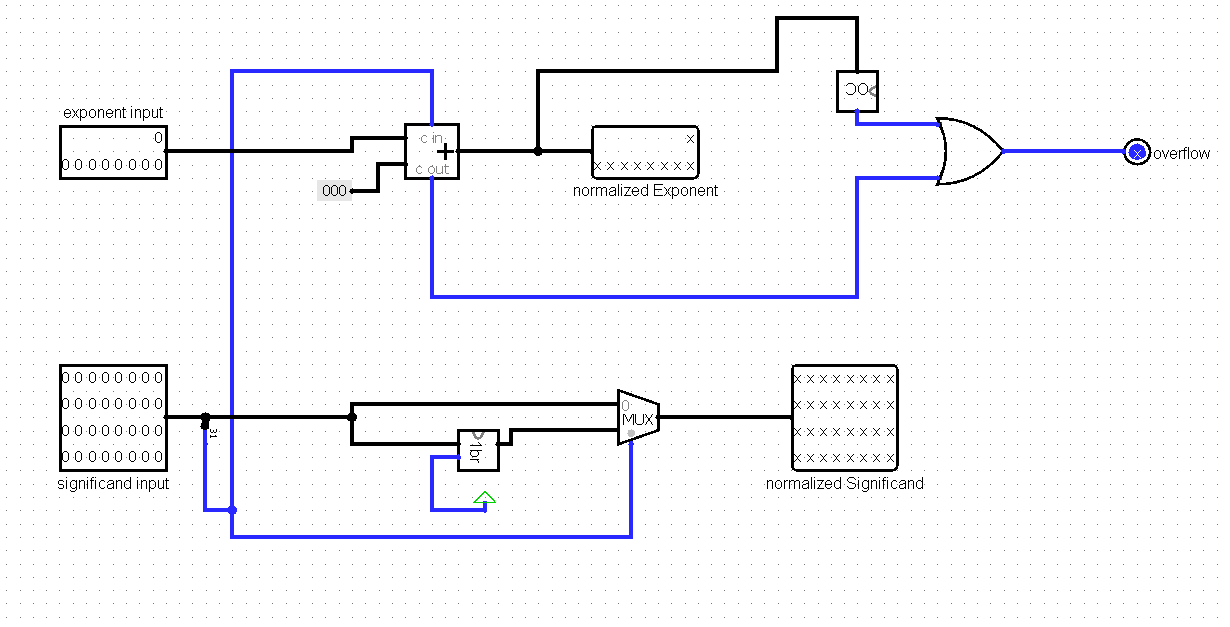
\includegraphics[width=\textwidth]{rounded_normalizer.png}
        \caption{Rounded-Normalizer}
    \end{subfigure}
    \begin{subfigure}[b]{0.3\textwidth}
        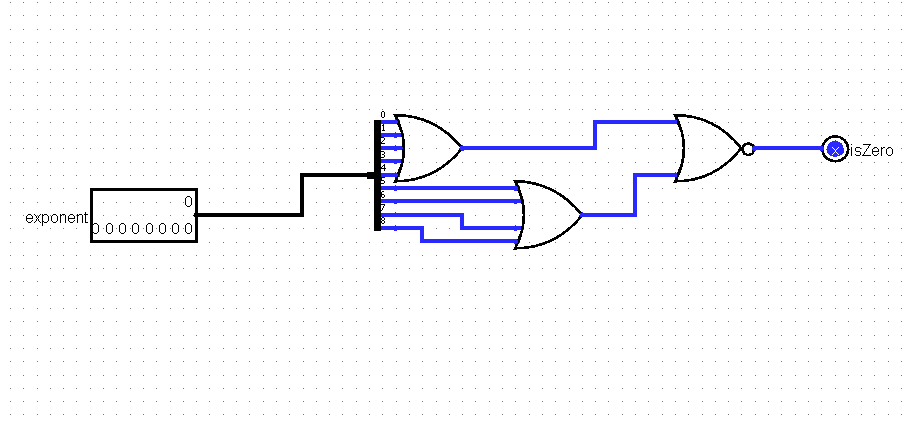
\includegraphics[width=\textwidth]{zero_checker.png}
        \caption{Zero-Checker}
    \end{subfigure}
    \begin{subfigure}[b]{0.3\textwidth}
        \includegraphics[width=\textwidth]{one_checker.png}
        \caption{One-Checker}
    \end{subfigure}
    
    \caption{Normalizer Circuits}
    \label{fig:normalizer_circuits}
\end{figure}




\subsection*{3.5 Rounding Circuit}
The \texttt{Rounder.circ} module is designed to handle the rounding of the mantissa in the floating-point adder. It integrates two main components to achieve precise rounding:

\begin{itemize}
    \item \textbf{Comparator:} This component evaluates specific bits of the mantissa to determine whether rounding is necessary.
    \item \textbf{Full Adder:} Based on the comparator's result, the full adder adjusts the mantissa to perform the rounding operation.
\end{itemize}


\begin{figure}[h!]
\centering
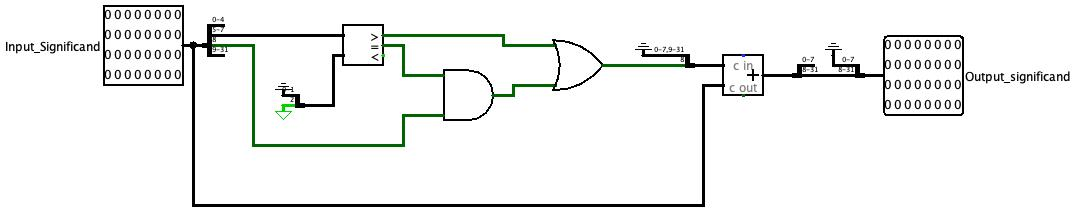
\includegraphics[width=0.8\textwidth]{Rounding.jpg} % Replace with actual image filename
\caption{Rounding Circuit module (\texttt{Rounder.circ}).}
\label{fig:rounding_circuit}
\end{figure}
\pagebreak


% \subsection*{3.6 Floating Point Adder}

% The final module, referred to as \texttt{FPA.circ}, integrates all the previously developed libraries and sub-modules to create the complete floating-point adder. This module implements the actual floating-point addition operation, or \textit{FPA}, by combining the sign, exponent, and mantissa components. The output processor, which consolidates these parts into the final result, is an essential part of this module. Additionally, the circuit is designed to handle special conditions like overflow and underflow, ensuring accurate and reliable computation.
\subsection*{3.6 Floating Point Adder}

The last module, called \texttt{FPA.circ}, uses the libraries and other modules to fully create a floating-point adder. It has the real floating-point adder, or circuit \textit{FPA}. The output processor circuit that merges the sign, exponent, and significand of the result is also included in this module.

\begin{figure}[h!]
    \centering
    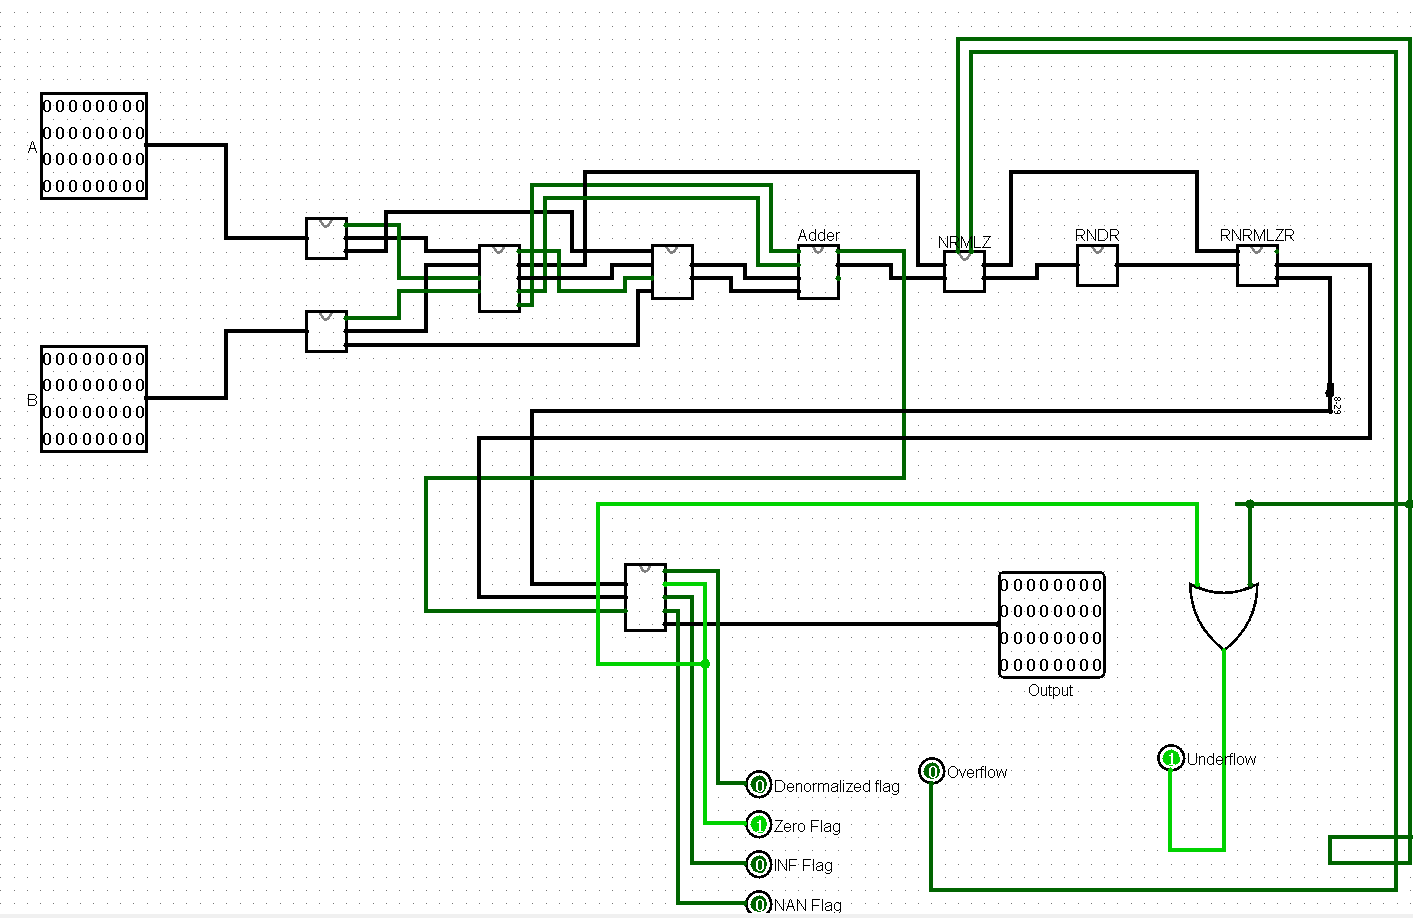
\includegraphics[width=0.8\textwidth]{FPA_Circuit.png} % Replace with the actual image file
    \caption{The FPA}
    \label{fig:fpa_circuit}
\end{figure}

\begin{figure}[h!]
    \centering
    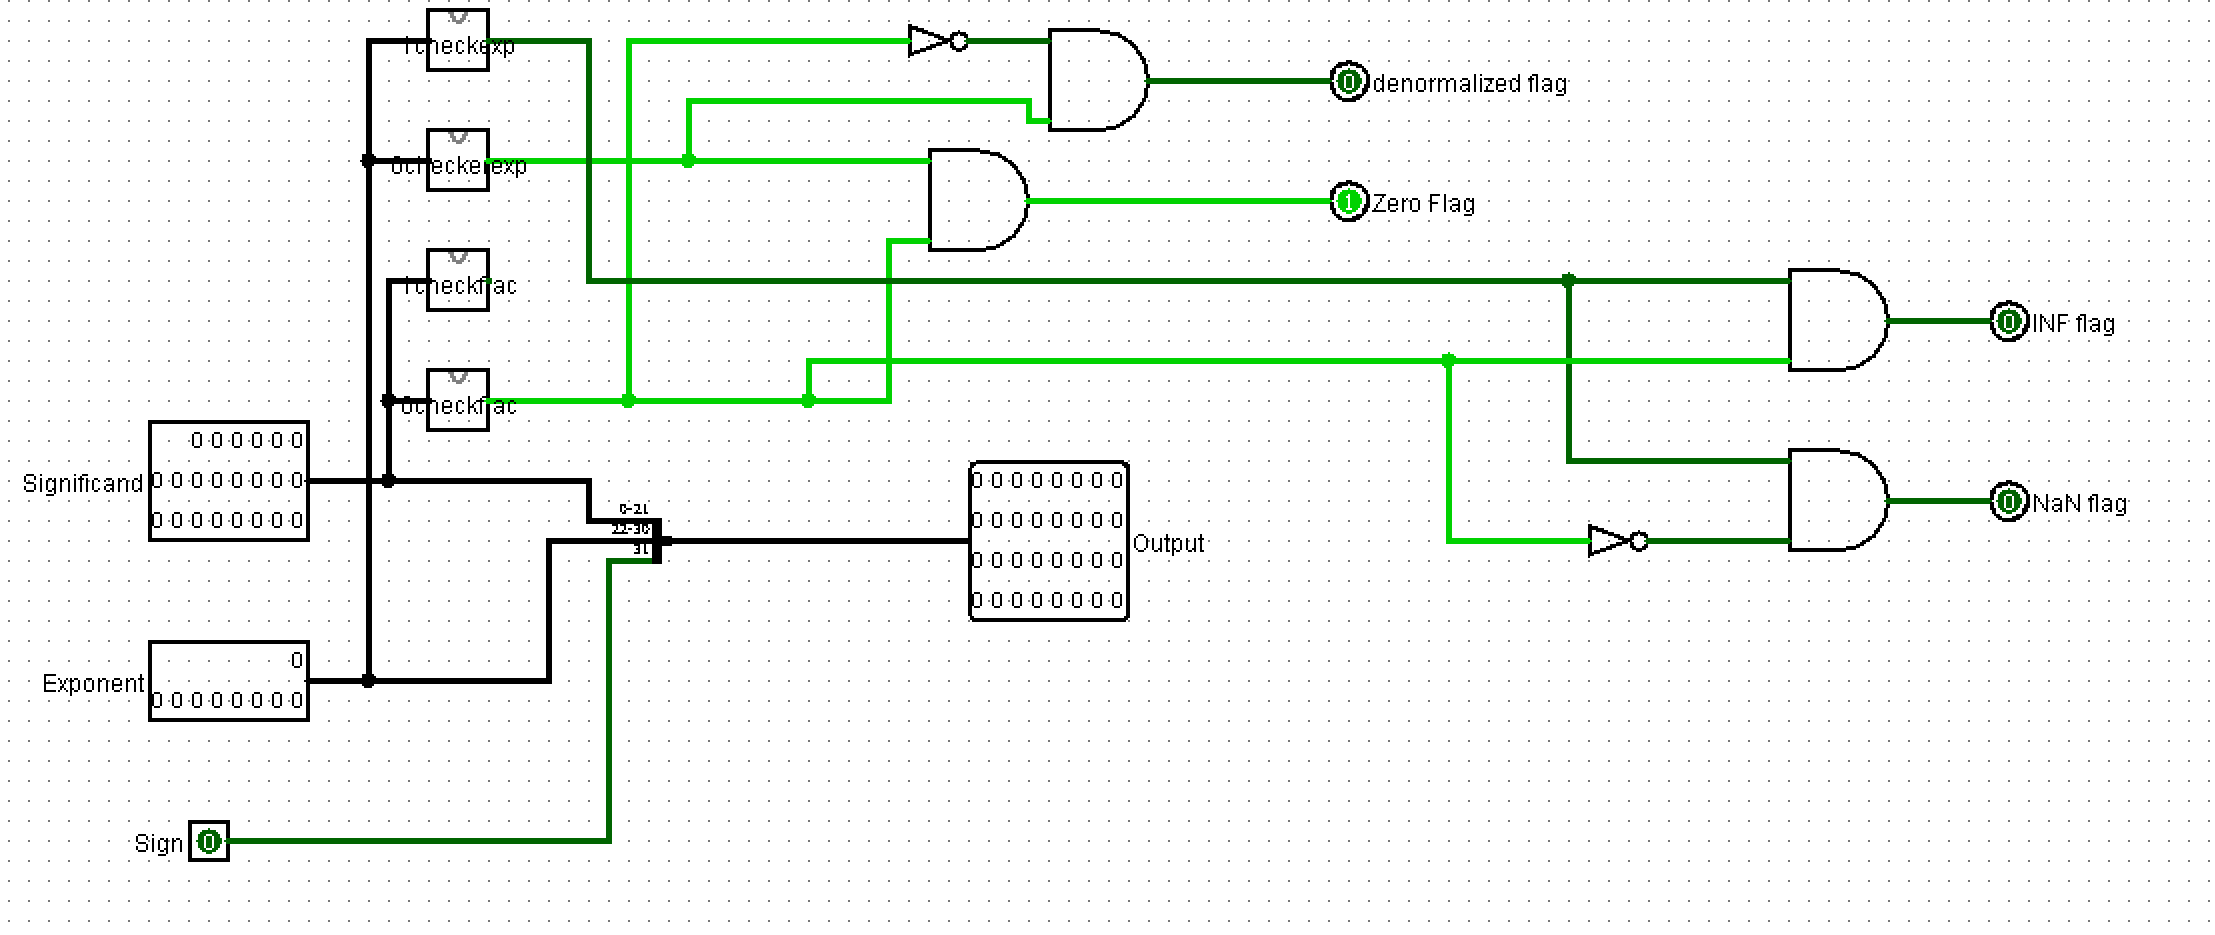
\includegraphics[width=0.8\textwidth]{outputhandler.png} % Replace with the actual image file
    \caption{Output Processor of the Result}
    \label{fig:output_processor}
\end{figure}







\subsection* {3.7 Third Party Libraries}
Third-party libraries \texttt{7400-lib.circ} and \texttt{logi7400dip.circ} are used to incorporate 7400 series ICs into the floating-point adder implementation. These libraries provide a modular and standardized approach for integrating logic gates and DIP IC models, ensuring efficient circuit design and compatibility.



\section*{4 Flowchart of the Addition/Subtraction Algorithm}

\begin{figure}[h!]
    \centering
    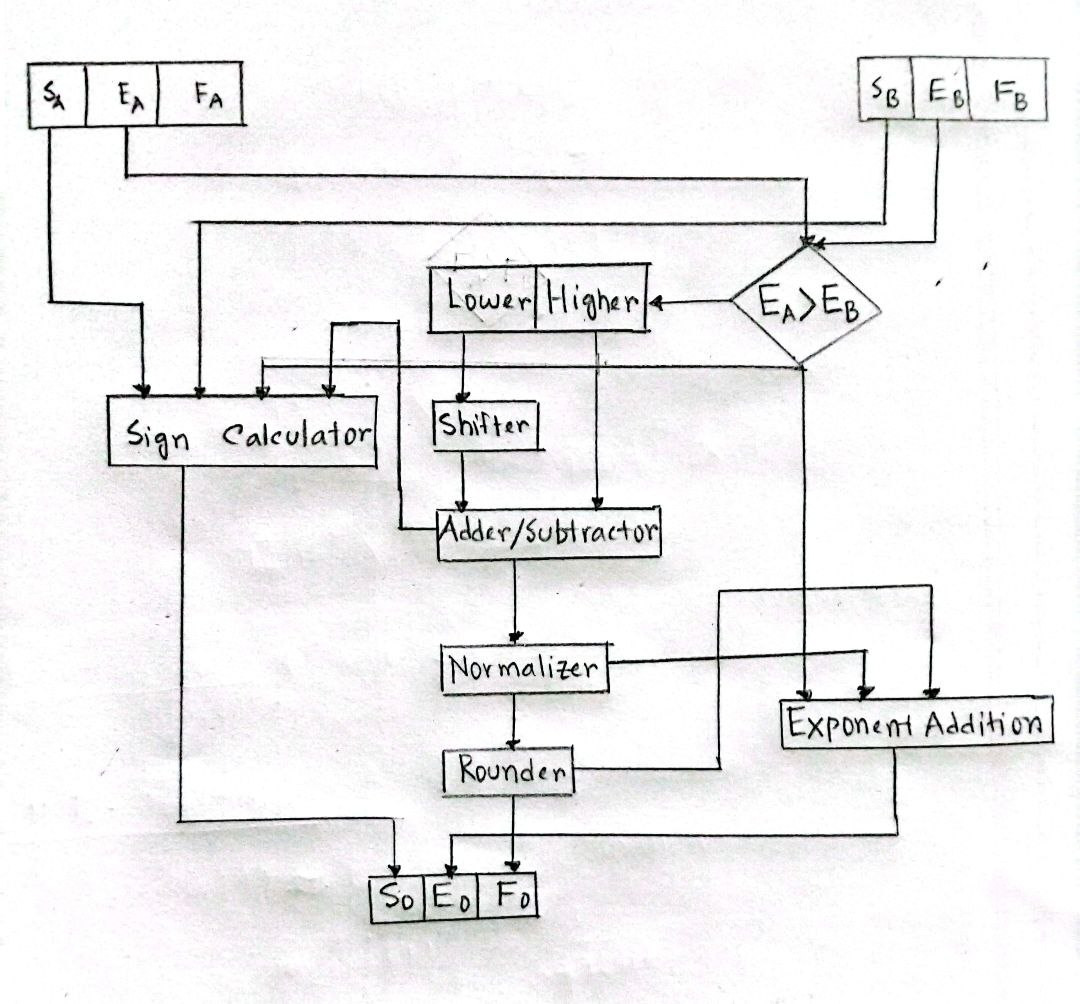
\includegraphics[width=0.8\textwidth]{flowchart.jpg}% Replace with your image file name
    \caption{Flowchart of the addition/subtraction algorithm}
    \label{fig:flowchart}
\end{figure}

% \section*{5 High-level Block Diagram of the Architecture}
% \begin{figure}[h!]
% \centering
% % Include your block diagram image here
% 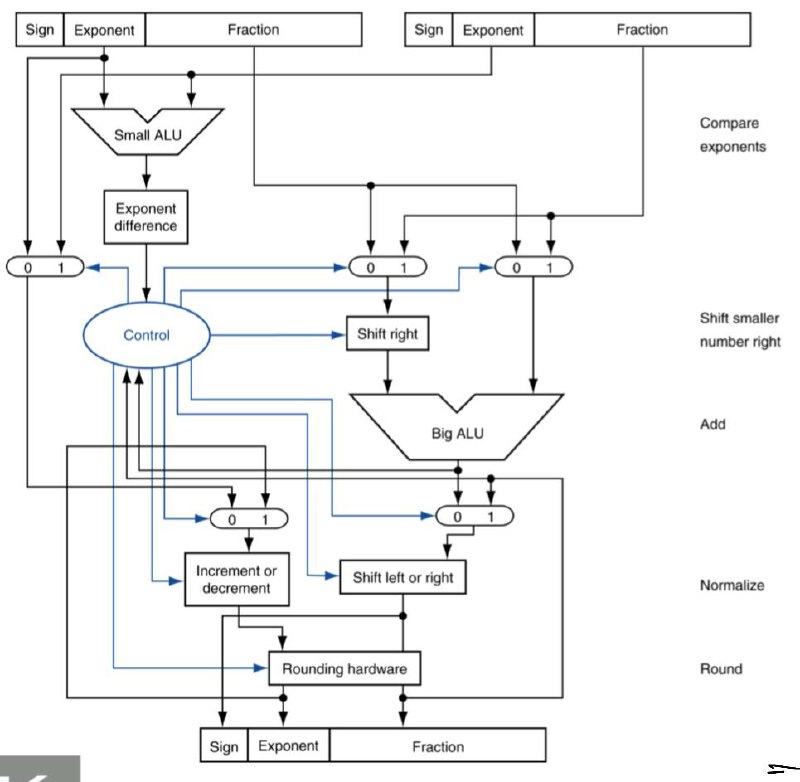
\includegraphics[width=\textwidth]{Block.jpg} 
% \caption{Block Diagram of the Floating Point Adder (FPA)}
% \label{fig:fpa_block_diagram}
% \end{figure}


% \begin{figure}[h!]
%     \centering
%     \includegraphics[width=0.9\textwidth]{fpa_circuit.png}
%     \caption{The Floating Point Adder (FPA)}
%     \label{fig:fpa_circuit}
% \end{figure}




% \section*{Flowchart of the Addition/Subtraction Algorithm}

% \begin{figure}[h!]
%     \centering
%     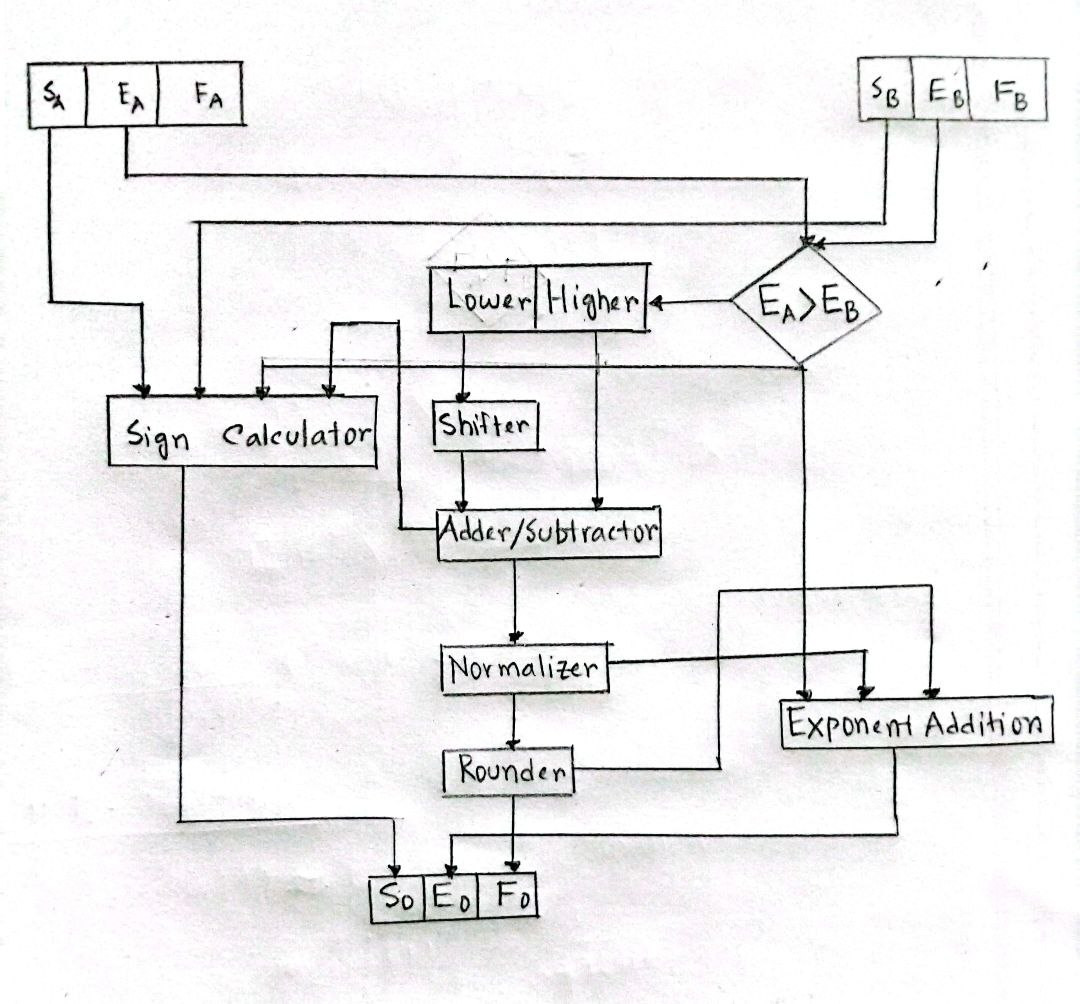
\includegraphics[width=0.8\textwidth]{flowchart.png} % Replace with your image file name
%     \caption{Flowchart of the addition/subtraction algorithm}
%     \label{fig:flowchart}
% \end{figure}


% \section*{5  High-level Block Diagram of the Architecture }





% \section*{Output}
% \begin{figure}[H]
%     \centering
%     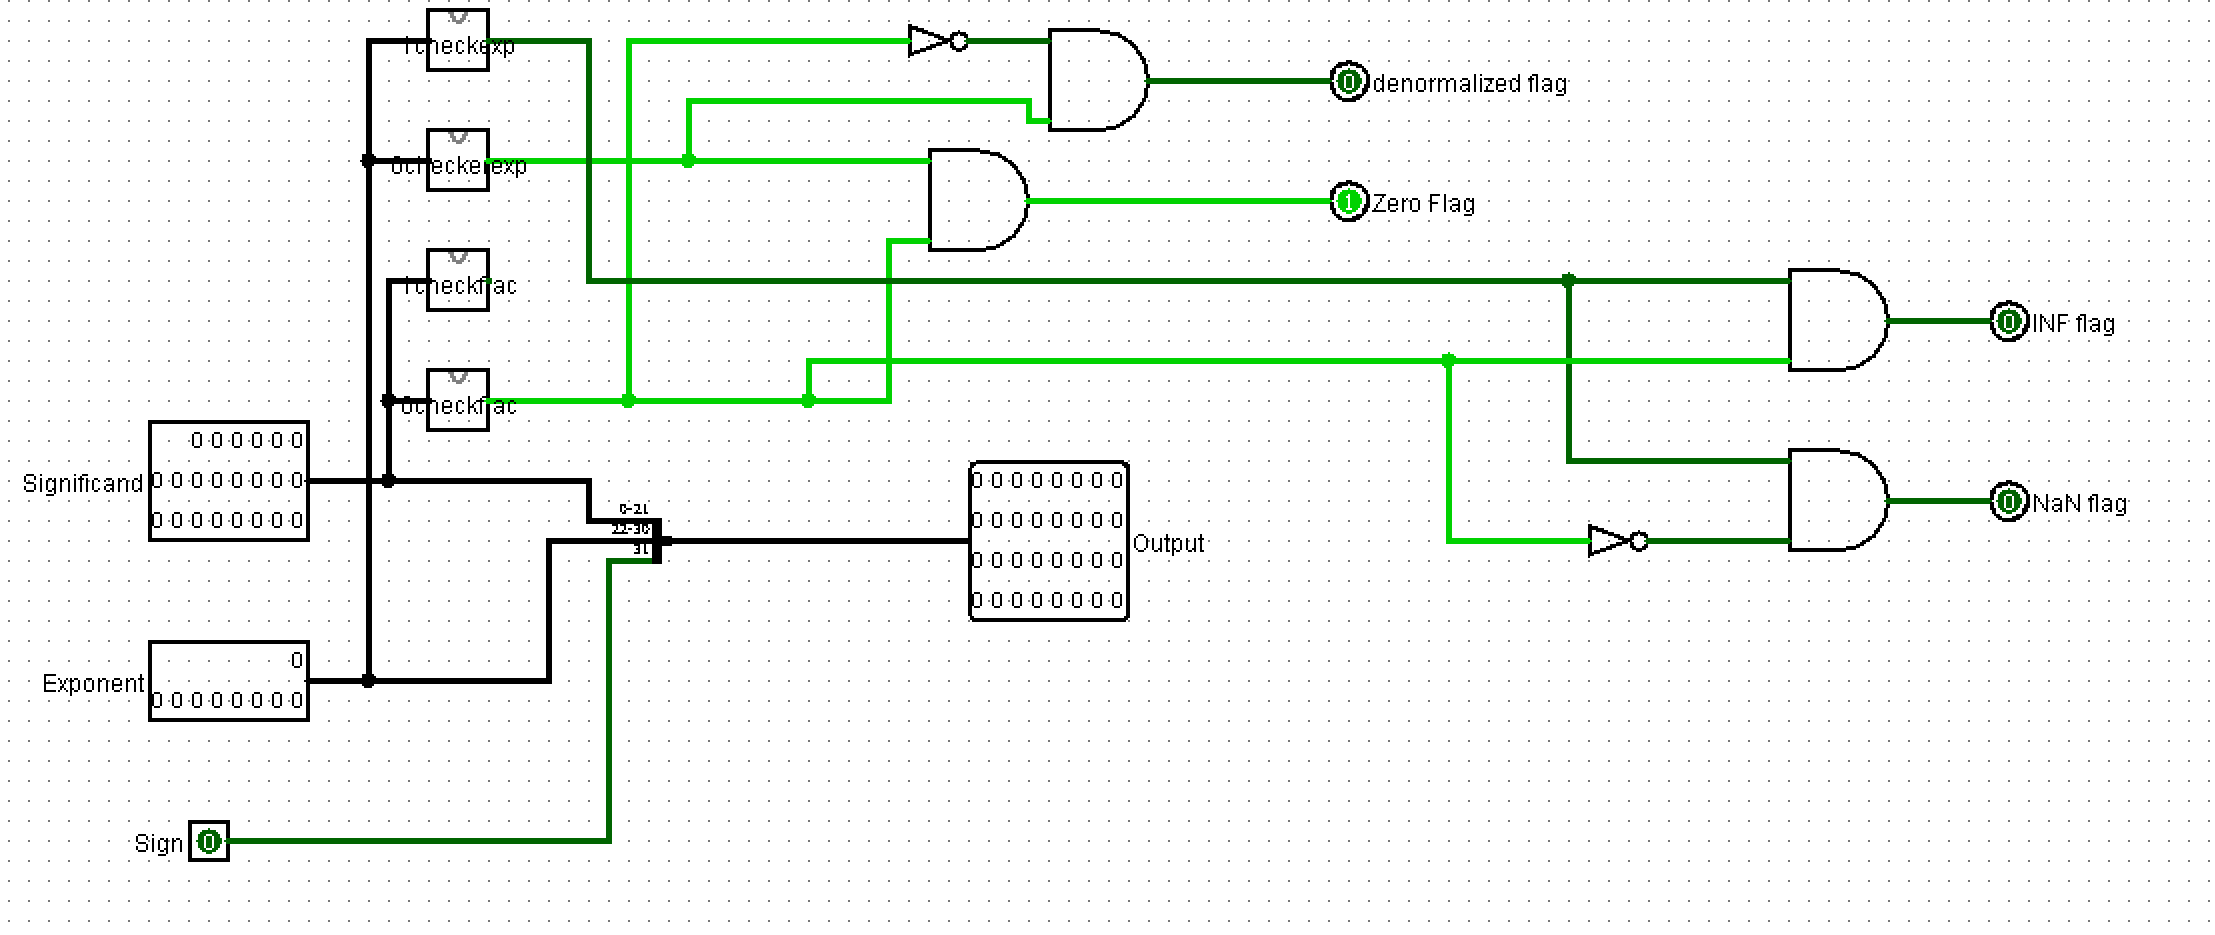
\includegraphics[width=0.8\textwidth]{outputhandler.png} % Replace with your image file name
%     \caption{32 Bit Adder Circuit}
%     \label{fig:Output Processor of the Resul}
% \end{figure}
\pagebreak

\section*{5 High-level Block Diagram of the Architecture}
\begin{figure}[h!]
\centering
% Include your block diagram image here
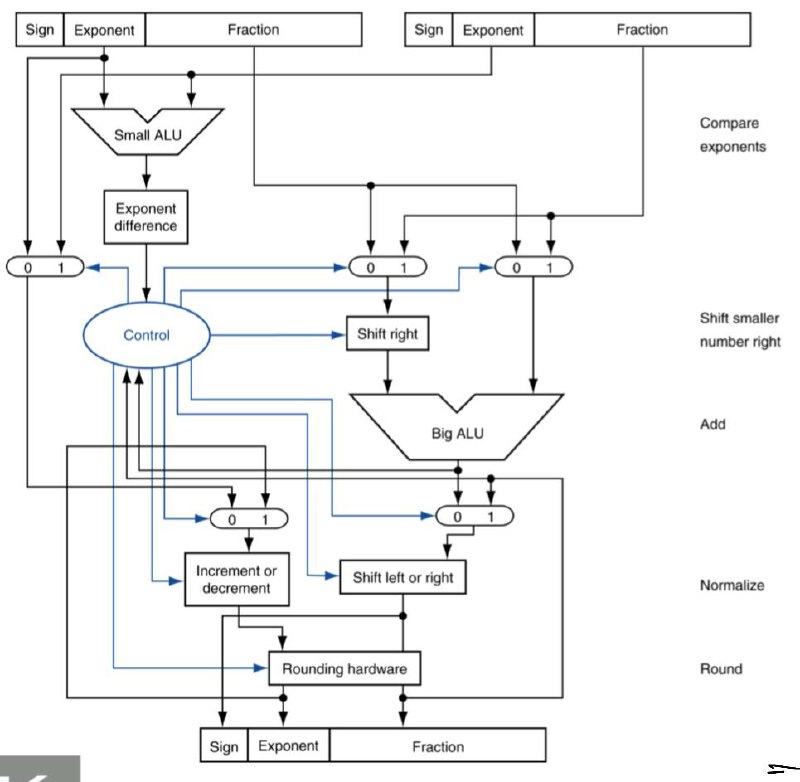
\includegraphics[width=\textwidth]{Block.jpg} 
\caption{Block Diagram of the Floating Point Adder (FPA)}
\label{fig:fpa_block_diagram}
\end{figure}
\pagebreak


\begin{figure}[H]
    \centering
    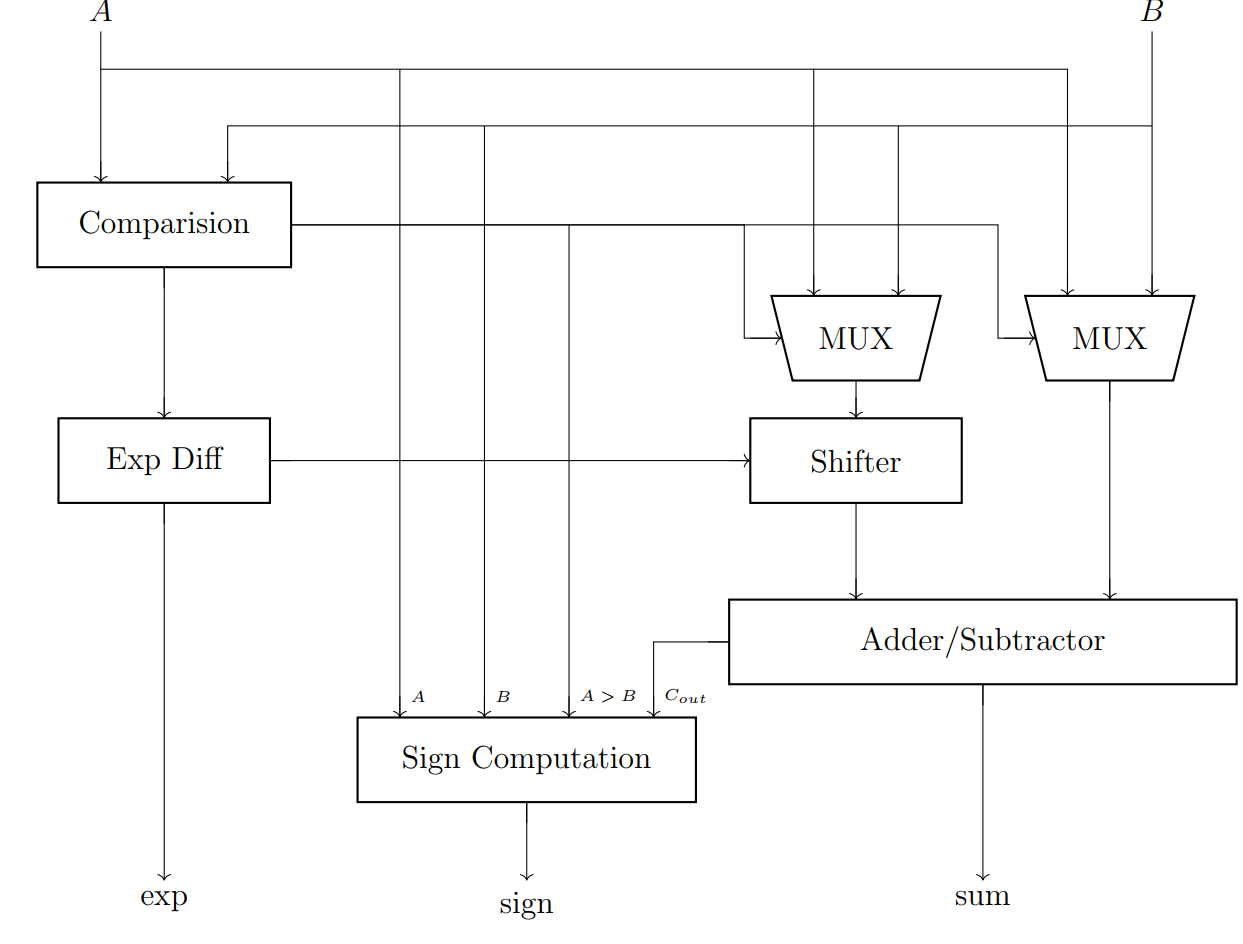
\includegraphics[width=0.8\textwidth]{blockadder.png} % Replace with your image file name
    \caption{Block Diagram of Added Input}
    \label{fig:Output Processor of the Resul}
\end{figure}



\section*{6. Comprehensive Design Description}

\subsection*{6.1 Comparing Exponents and Aligning the Radix Point}

To add two floating-point numbers, it is essential to align their radix points. This process ensures that both numbers are in the same scale before performing the addition. Typically, the alignment is achieved by shifting the number with the smaller exponent to the right. The difference between the exponents of the two numbers is calculated to determine the required number of shifts.

In our implementation, we utilized a subtractor to compute the difference between the two exponents, allowing for accurate alignment. The exponents are compared using a comparator to identify which input has the larger exponent. This ensures proper handling of the inputs and precise alignment of the radix points before proceeding to the addition stage.

\subsection*{6.2 Multiplexer-Based Shifting Mechanism}
The shifting process is implemented using a series of multiplexer-based shifters. Specifically, five 32-bit multiplexers are employed, each capable of performing shifts of 1, 2, 4, 8, or 16 bits. By combining these multiplexers, it is possible to achieve shifts of any length up to 31 bits. 

In cases where the required shift exceeds 31 bits, all bits of the smaller number are cleared to 0, effectively aligning it with the larger number. The input to the shifter circuit is derived from the exponent difference. To ensure accurate shifting, the lower five bits of the exponent difference are utilized while the upper seven bits are ignored. This design ensures that the maximum shift length does not exceed 31 bits (2\textsuperscript{5} - 1). If a larger shift is required, the fraction is cleared entirely, resulting in an output of zero.



\subsection*{6.3 Exponent Comparison and Radix Point Alignment}
To perform addition of two floating-point numbers, it is essential to align their radix points. This alignment is achieved by shifting the number with the smaller exponent to the right until it matches the larger exponent. The difference between the two exponents is calculated using a 9-bit subtractor, while a comparator determines which exponent is larger and the amount of shift required for proper alignment.
\subsection*{6.4 Rounding}
In our design, we use a 32-bit adder to perform the necessary additions and subtractions on the mantissas. However, since only 22 bits can be stored, sometimes rounding is required. The 23rd bit is reserved as the guard bit, and the 24nd bit is used for rounding. If any bits beyond the round bit are set, we activate the sticky bit. If no additional bits are set, the sticky bit remains inactive. We need to consider the following scenarios when performing rounding:

\begin{table}[h!]
\centering
\begin{tabular}{|c|c|c|c|c|}
\hline
\rowcolor{gray!20} \textbf{22nd bit} & \textbf{G} & \textbf{R} & \textbf{S} & \textbf{Action} \\ \hline
\rowcolor{white} X & 0 & X & X & Truncate \\ \hline
\rowcolor{gray!10} 1 & 1 & X & X & Round up \\ \hline
\rowcolor{white} 0 & 1 & 0 & 0 & Truncate \\ \hline
\rowcolor{gray!10} X & 1 & 1 & X & Round up \\ \hline
\rowcolor{gray!10} X & 1 & X & 1 & Round up \\ \hline
\end{tabular}
\caption{Rounding Behavior Based on Bits}
\end{table}
\noindent
\textbf{Note:} Truncation occurs only when the value of GRS is \( 100 \). Additionally, if the 22nd bit is 1, then 1 is added; otherwise, 0 is added.
K map for the whole process is give below :


\subsection*{6.5 Computing the Sign Bit}

When computing the sign bit, there are a few things to keep in mind. The sign of the output will be either of the inputs' signs if the signs of the two inputs are the same. In the event they differ, we must take two factors into account. First, we must determine the adder's output sign. It can be calculated using the equation:

\begin{equation}
    \text{sign} = (S_A \oplus S_B)\overline{C_{\text{out}}}
\end{equation}

Where $C_{\text{out}}$ is the carry out of the adder. Since we constantly deduct the input with the smaller exponent from the input with the higher exponent, this sign could not always be accurate. $1$ yields the opposite result to the right one when the signs of the inputs are opposite, that is, if the input with the larger exponent is negative and the other one is positive. We have included a variable \textit{switch} to address this. In some situations, this switch bit will change the sign bit. When the inputs' sign bits are opposite and the input with the larger exponent is negative, our sign bit will fail. The switch will then become $1$ and change the sign in that scenario. The switch bit equation is:

\begin{equation}
    \text{switch} = (S_A \oplus S_B)(\text{Comp} \oplus S_B)
\end{equation}

Here, \textit{Comp} is the output of the comparator circuit $(Exp_A > Exp_B)$. So, the formula for the actual sign bit:

\begin{equation}
    \text{actualSign} = \text{sign} \oplus \text{switch}
\end{equation}

If there are differences in the signs of the inputs, equation (3) will be applied. If not, the output's sign will be directly affected by the first input's sign. A multiplexer will be used to make this choice.

\subsection*{6.6 Handling Zero or Small Input}

The other input will be sent directly to the output if one of the inputs is zero. Furthermore, the input with the larger exponent passes directly to the output if the exponent of one of the inputs is substantially smaller than the other (a difference of greater than $31$).


\subsection*{6.7 Enhancing Precision}
In our design, we chose not to allocate a separate bit for capturing the overflow. Instead, we directly extracted this information from the carry-out. Additionally, we did not require a separate bit to indicate the sign during subtraction. Instead, the sign of the result was determined by examining the carry-out of the adder. If the carry-out is 1, the result is positive; if it's 0, the result is negative. Special handling is required when one of the summands is zero, which, as discussed in section 6.6, is dealt with separately. This approach effectively increases the precision by 2 bits.


\section*{7. ICs Used with Count}

The following table lists the ICs used in the design, along with their respective quantities:

\begin{table}[h!]
\centering
\begin{tabular}{|c|c|}
\hline
\textbf{IC} & \textbf{Quantity} \\ \hline
IC 7404 & 1 \\ \hline
IC 7408 & 5 \\ \hline
IC 7432 & 4 \\ \hline
IC 7486 & 1 \\ \hline
IC 74157 & 7 \\ \hline
\textbf{Total} & \textbf{18} \\ \hline
\end{tabular}
\caption{ICs Used with Quantity}
\end{table}

\noindent
The IC count is relatively low because we used Logisim's built-in libraries for adders , comparators and shifters , eliminating the need to design them from scratch or count their ICs.
Even above gate has not been used in IC gate formate rather Basic gate.
\section*{8. Simulator Used and Version}
The floating point adder circuit was simulated using Logisim version 2.7.1.

% \end{document}






\section*{9 Discussion}

Designing the floating-point adder (FPA) circuit was both a challenging and rewarding experience. Instead of tackling the entire circuit as one complex block, we adopted a modular approach by dividing the design into smaller sub-modules. This strategy not only helped streamline the workload among group members but also allowed us to test and debug individual components more effectively.

One of the primary challenges we encountered was constructing a shifter capable of handling variable shift amounts. To address this, we implemented a cascading approach using shifters for 1, 2, 4, 8, and 16 bits, each corresponding to a specific input bit in the shift control. This modular implementation allowed for greater flexibility and reusability across the design.

Another significant challenge was dealing with negative inputs. We realized that the output behavior depended heavily on the signs and magnitudes of the inputs. After analyzing possible scenarios, we identified four unique cases and developed a solution using a combination of adders, subtractors, XOR gates, and multiplexers. This approach simplified the handling of signed inputs without compromising performance.

Overflow and underflow management posed yet another challenge. Instead of reserving a dedicated bit for overflow or underflow, we leveraged the carry-out bit from the adder to detect such conditions. This optimization allowed us to increase the precision of our design by utilizing the additional bits for computation, improving overall efficiency.

We also made use of built-in circuits available in the simulation library to complement our custom-designed modules. This integration of prebuilt components with our design ensured a minimalist yet fully functional floating-point adder while adhering to the IEEE 754 standard.

Overall, this project provided valuable insights into the complexities of floating-point arithmetic and circuit design. By overcoming these challenges, we gained a deeper understanding of the theoretical and practical aspects of building a robust floating-point adder, which has wide applications in modern computing systems.



\end{document}

